% ch13b Disorder: localization and exceptions, part b (书页 275-288 / 分册p018-031)
\section{局域化的例外}

在 $d=1,2$ 中不存在载流态（current-carrying states），是无序体系中最真正令人惊讶的结果之一。正如上一节所述，当时间反演对称性被破坏时，载流态可以在低维中存留。然而，即便时间反演对称性完好无损，局域化原理仍然存在三个重要的例外：（1）无序彼此关联的无规二聚体模型；（2）薄膜中的绝缘体--超导体转变；（3）新近在稀薄二维电子气中发现的导电态。本节将对三者逐一评述，不过对后两者的讨论将从简。

\subsection{无规二聚体模型}

在迄今讨论的模型中，格点能量或矩阵元都是从单一无规分布中抽取的、严格统计独立的量。然而在任何真实物理体系中，格点能量与矩阵元是彼此关联的。直到 20 世纪 80 年代中期，关于统计关联在局域化转变中所起作用的研究（JK1986）仍然出奇地少，部分原因在于人们怀疑真实体系中天然存在的关联根本无法以任何方式确定地给出，因而所提模型的物理意义也就不清楚。例如，考虑线性链上最近邻紧束缚哈密顿量的格点幅所满足的本征值方程
\begin{equation*}
E c_{n}=\epsilon_{n}c_{n}+V_{n,n+1}c_{n+1}+V_{n,n-1}c_{n-1}\tag{13.37}
\end{equation*}
当 $-\epsilon_{n}=V_{n,n+1}+V_{n,n-1}$ 时，本征值方程约化为
\begin{equation*}
E c_{n}=V_{n,n+1}(c_{n+1}-c_{n})+V_{n,n-1}(c_{n-1}-c_{n}),\tag{13.38}
\end{equation*}
它在形式上与具有无规近邻跳跃速率的概率扩散方程完全相同。众所周知，该方程在 $E=0$ 处有一个扩散极点；也就是说，$E=0$ 的态是扩展态（A1981）。因此，这里这个关联无序的简单模型具有一个扩散模式。除结构无序的情形外，导致式 (13.38) 的这种关联在电子层面上充其量是人造的。弗洛雷斯（Flores）（F1989）探索了格点能量与矩阵元之间其他形式的代数关联，发现有无穷小比例的电子态具有零反射系数，因而在一维中是扩展的。鉴于前文给出的、禁止一维存在扩展态的标度论证，这一结果着实令人惊讶。

为理解一维体系拥有扩展态所必须满足的最低物理条件，我们考虑由邓拉普（Dunlap）、吴（Wu）与菲利普斯（Phillips）（DWP1990）引入的模型，称为无规二聚体模型（random dimer model，RDM）。为给 RDM 提供背景，考虑无规二元合金。在无规二元合金的紧束缚模型中，格点能量 $\epsilon_{a}$ 与 $\epsilon_{b}$ 分别以概率 $p$ 与 $1-p$ 随机地指派到格点上。一个常数的近邻矩阵元 $V$ 传递格点之间的输运。该模型中所有的态都是局域的。无规二元合金中一个典型波函数示于图 13.2。把二元合金中所有含奇数个 $\epsilon_{b}$ 的团簇替换为含相同数目 $\epsilon_{a}$ 的团簇，便得到 RDM。所得结果是一个 $b$ 缺陷随机出现但成对出现的无规晶格。RDM 泛指任何至少有一种格点能量被随机指派到成对格点上的晶格。RDM 中一个典型的二聚体示于图 13.9。RDM 令人惊讶的特征是：有 $\sqrt{N}$ 个电子态在整个样品中保持扩展，只要 $-1\le W\le 1$，其中
\begin{equation*}
W=\frac{\epsilon_{a}-\epsilon_{b}}{2V}.\tag{13.39}
\end{equation*}

\begin{figure}[H]\centering
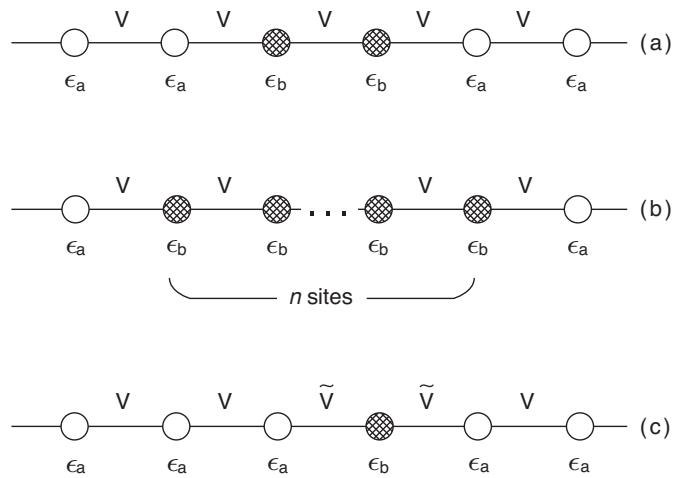
\includegraphics[width=0.7\textwidth]{figs/ch13/fig_13.9.jpg}
\caption*{图 13.9\quad （a）RDM 中的二聚体缺陷；（b）具有二聚体对称性的 $n$ 格点缺陷；（c）排斥性二元合金中的缺陷。}\label{fig:auto:13.9}
\end{figure}

RDM 的另一个特点是：只要 $-1<W<1$，初始局域的粒子的均方位移便按 $t^{3/2}$ 超扩散地增长。只有当无序增大到 $W=\pm 1$ 时才得到通常的扩散。在所有其他情形下，粒子在长时间后仍是局域的。至少存在扩散输运，这一关键特征保证了 RDM 的确构成一个反例，否定了禁止一维长程输运的标度论证。

理解 RDM 的最简单方式，是计算放在一个除它之外完全有序、晶格常数为 1 的晶格中的单个二聚体的反射系数。把二聚体放在格点 0 与 1 上，能量为 $\epsilon_{b}$；所有其他格点指派能量 $\epsilon_{a}$。为计算反射幅（$R$）与透射幅（$T$），把格点幅写作
\begin{equation*}
c_{n}=\begin{cases}\mathrm{e}^{\mathrm{i}kn}+R\,\mathrm{e}^{-\mathrm{i}kn}, & n\le-1,\\ T\,\mathrm{e}^{\mathrm{i}kn}, & n\ge 1\end{cases}\tag{13.40}
\end{equation*}
其中 $k$ 是无量纲波矢。把式 (13.40) 代入格点 1 与 $-1$ 的本征值方程即式 (13.37)，便可确定原点处的格点幅。结果是 $c_{0}=1+R=T(\epsilon_{-}\mathrm{e}^{-\mathrm{i}k}+V)/V$，其中 $\epsilon_{-}=\epsilon_{a}-\epsilon_{b}$。再把这一结果代入格点 0 的本征值方程，便得到反射概率的闭式表达式
\begin{equation*}
|R|^{2}=\frac{(W+\cos k)^{2}}{(W+\cos k)^{2}+\sin^{2}k}\tag{13.41}
\end{equation*}
于是我们看到，当 $W=-\cos k$ 时反射系数为零；只要 $-1\le W\le 1$，总会有某个 $k$ 值满足这一条件。完美透射的电子态在母有序带中的位置对应于波矢 $k_{\mathrm{o}}=\cos^{-1}W$。在 $k_{\mathrm{o}}$ 处，有序带与无序带没有差别；两者的态密度在这一点重合。单个二聚体在特定能量下反射系数为零，可以理解为一种共振效应：二聚体起着共振腔的作用。在特定波矢 $k_{\mathrm{o}}=\cos^{-1}W$ 处，来自二聚体第二个格点的反射与来自第一个格点的反射相位差 180°。在这个能量下，透射系数为 1。

考虑无序的情形。由于穿过单个二聚体的透射系数为 1，无规二聚体的具体分布不应影响完美透射的态。事实的确如此，可以从如下论证看出。穿过 RDM 任意一段的输运可以表示为 $\cdots T_{a}^{n_{1}}T_{b}^{2n_{2}}T_{a}^{n_{3}}T_{b}^{2n_{4}}\cdots$，其中 $n_{i}$ 是随机变量，$T_{n}$ 是转移矩阵。注意 $b$ 转移矩阵出现的次数全为偶数，这就是二聚体约束。由格点幅的本征值方程即式 (13.37)，转移矩阵为
\begin{equation*}
\begin{pmatrix} c_{n+1}\\ c_{n}\end{pmatrix}=\begin{bmatrix}\dfrac{E-\epsilon_{n}}{V} & -1\\[4pt] 1 & 0\end{bmatrix}\begin{pmatrix} c_{n}\\ c_{n-1}\end{pmatrix}=T_{n}\begin{pmatrix} c_{n}\\ c_{n-1}\end{pmatrix}.\tag{13.42}
\end{equation*}
共振条件 $W=-\cos k$ 等价于 $E=\epsilon_{b}$，因为 $E$ 是有序带的能量。在这个能量下，跨越一个 $b$ 缺陷的转移矩阵约化为
\begin{equation*}
T_{b}=\begin{bmatrix} 0 & -1\\ 1 & 0\end{bmatrix}.\tag{13.43}
\end{equation*}
该矩阵的平方（对应于跨越一个 $b$ 二聚体的转移矩阵）是单位矩阵的负值。于是在共振时，RDM 中转移矩阵的乘积彼此对易，$b$ 二聚体可以被简单地抹去，只付出一个符号改变的代价。因此，穿过一个二聚体缺陷的相移为 $\Omega=-2k+\pi$。无散射态对应于这样一个布洛赫态：二聚体格点实际上已被消去，代价是在二聚体格点处引入相移。因此，电子一旦穿过单个二聚体缺陷，就不会再被任何其他二聚体缺陷散射，因为无论放置在何处，所有二聚体都具有完全相同的共振条件。若二聚体放在格点 0、1 和 2、3 上，则无散射态为
\begin{equation*}
\ldots,\mathrm{e}^{-2\mathrm{i}k},\mathrm{e}^{-\mathrm{i}k},1,-\mathrm{e}^{-\mathrm{i}k},-1,\mathrm{e}^{-\mathrm{i}k},1,\mathrm{e}^{2\mathrm{i}k},\ldots.\tag{13.44}
\end{equation*}
这样的一个无散射态的例子绘于图 13.10。

当然，如果只有一个电子态保持无散射，是不会有输运的。为确定在整个样品上扩展的态的总数，我们把 $R$ 在 $k_{\mathrm{o}}$ 附近展开。到最低阶，我们发现 $k_{\mathrm{o}}$ 附近 $|R|^{2}\propto(\Delta k)^{2}$，其中 $\Delta k=k-k_{\mathrm{o}}$。散射事件之间的时间 $\tau$ 反比于反射概率。因此，$k_{\mathrm{o}}$ 附近的平均自由程 $\ell=v_{\mathrm{F}}\tau\propto 1/(\Delta k)^{2}$。令平均自由程等于系统长度 $N$，我们发现平均自由程等于系统大小的态的总数（$\Delta N$）按 $\Delta N=\sqrt{N}$ 标度。由于在一维中平均自由程与局域化长度相等，我们得出局域化长度发散的态的总数为 $\sqrt{N}$。这里给出的单二聚体论证已被博维耶（Bovier）（B1992）证明对无规体系同样成立。博维耶的论证尤为优雅，它严格地确立了李雅普诺夫指数（Lyapunov exponent，局域化长度的倒数）在共振 $k_{\mathrm{o}}=\cos^{-1}W$ 附近（作为 $\Delta k_{\mathrm{o}}$ 的函数）按二次方式消失。因此，在 RDM 中有 $\sqrt{N}$ 个电子态在整个样品长度上保持扩展。

\begin{figure}[H]\centering
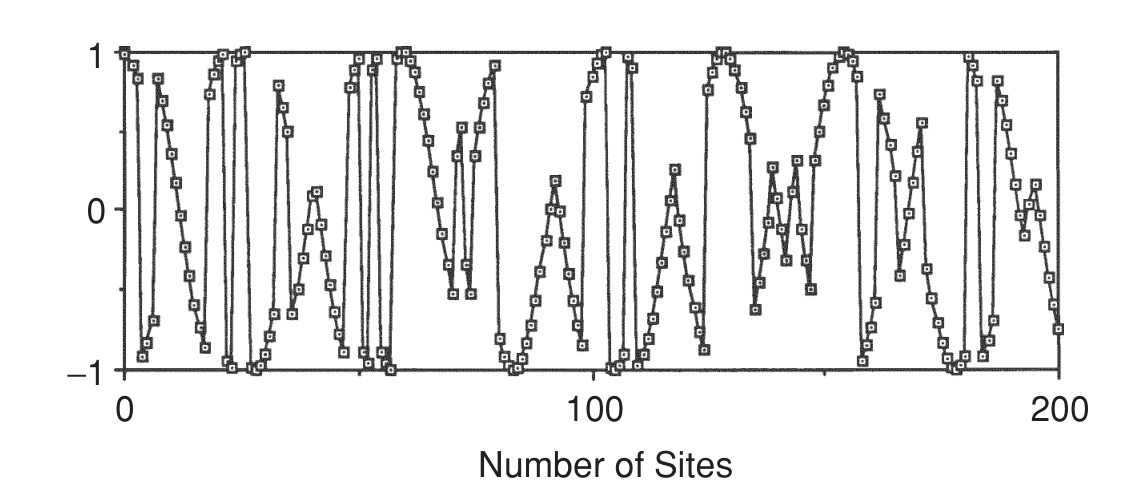
\includegraphics[width=0.6\textwidth]{figs/ch13/fig_13.10.jpg}
\caption*{图 13.10\quad 无规二聚体模型中一个典型扩展态的实部。}\label{fig:auto:13.10}
\end{figure}

这些态最终会对输运性质作出贡献。由于 RDM 中扩展态的平均自由程至少是系统大小，这些态以恒定的群速度 $[v(k)]$ 在晶体中弹道式地运动，除非它们位于速度为零的带底或带顶。由于所有其他电子态都是局域的，我们通过在参与输运的态的宽度上积分 $v(k)\ell(k)$ 来确定扩散常数。积分的上限于是正比于未散射态的总比例，即 $\ell(k)/\sqrt{N}$，而 $\ell(k)\approx N$。当速度为非零常数时，我们得到 $D\approx\sqrt{N}$。由于对输运有贡献的态以恒定速度走过系统的长度，它们经过的距离按时间的线性函数标度。因此 $N\propto t$，且 $D\approx t^{1/2}$，从而均方位移按 $t^{3/2}$ 增长。在群速度为零的带底或带顶处，$v(k)\propto k$，而 $D\propto O(l)$。这表明 RDM 中狭窄的扩展态带足以使初始局域的粒子退局域化。如此少的态竟能起如此大的作用，这确实是 RDM 的一个奇特之处。

尽管如此，RDM 与基于自能虚部的局域化判据完全相容。按照这一判据，若当 $E$ 逼近实轴时 $\mathrm{Im}\,S(E)\to 0$，则本征态是局域的。$\mathrm{Im}\,S(E)$ 只有在 $G(E)$ 具有虚部，即等价地具有分支点奇异性时才非零。在热力学极限下，无穷小数目的扩展态不足以产生具有非零宽度的割线。因此在 RDM 中，$\mathrm{Im}\,S(E)$ 对所有能量都为零。自能局域化判据对零测度的扩展态集合不敏感。令人惊讶的是，这些态的数目却足以产生长程输运。彭德里（Pendry）（P1987）证明，在标准的无序模型中，特定能量上的孤立态可以在 $\sqrt{N}$ 个格点上保持扩展。然而，以这种方式表现的态的数目是指数小的，因而无关紧要。

RDM 的实质在于：在带内某个能量处，缺陷的转移矩阵约化为单位矩阵的负值（WGP1992）。因此在二聚体共振处，完美透射从样品的一侧直达另一侧。局域的二聚体关联创造了这一宏观量子效应。容易证明，这一结果只在二聚体的两个格点能量相等，即二聚体对称时才成立。对称面是缺陷拥有共振态的充要条件。可以作出的普遍表述如下：只要缺陷包含一个对称面，无序\emph{使电子态局域化的标准倾向就会在带内某些能量处受到抑制}。这是一维中扩展态得以存在的最低要求。RDM 只是缺陷拥有对称面的最简单模型；任何无规 $n$ 聚体都足够，如图 13.9(b) 所示。此外，图 13.9(c) 所示的单缺陷模型是 RDM 的非对角对偶（off-diagonal dual），类似的退局域化也出现在该模型中（P1993）。这类简单的关联无序模型至今仍是活跃的研究领域。事实上，在人为构筑了 RDM 关联的 GaAs/AlGaAs 异质结构中开展的实验（B1999），已经证实了无规二聚体模型中扩展态的存在。

\subsection{绝缘体--超导体转变}

在第二类例外中，局域化被强电子相互作用所挫败。在第一种情形中，我们考虑薄膜中从绝缘体到超导体的转变。虽然单个电子会被无序局域化，但形成库珀对的电子在二维中可以退局域化。实验上，已经在二维中通过两种不同的机制观察到从超导体到绝缘体的直接转变。第一种是简单地减小样品的厚度（J1989；GM1998）。这实际上改变了散射长度，因而等价于改变无序的数量。结果，库珀对在整个转变过程中保持完好；然而在绝缘体中它们是局域的，而在超导体中它们形成相干态。为理解库珀对如何在绝缘与超导两个极端之间被调节，考虑图 13.11。如图 13.11 所示，库珀对的形成并不是超导电性的充分条件。如果设想把薄膜划分为若干分区（如图 13.11 所示），那么当每个分区在每一时刻的快照中都具有相同数目的库珀对时，就得到绝缘行为；也就是说，这个态是静态的。然而，若库珀对数目在分区之间涨落，库珀对的输运就成为可能，从而得到超导电性。如第 12 章所示，在超导体中相位与粒子数是共轭变量。若相位是锐定的，则粒子数完全不确定；同样，粒子数的完全确定导致相位的无穷不确定。然而，相位相干的破坏会压制超导电性。因此，当调节某个外部参量使全局相位相干得以建立时，就发生从库珀对绝缘态到超导态的转变。膜厚或无序就是这样一种参量。在临界点上，电阻率将与温度无关。因此，正处于失去全局相位相干边缘的库珀对，在零温下获得有限的电阻率，如同金属那样。这一点特别重要，因为它表明被限制在一个平面上的库珀对有三种可能（J1989；GM1998；F1990）：（1）电阻率无穷大的绝缘体；（2）电阻率消失的超导体；（3）零温下电阻率有限的金属。对单个电子而言只有第一种可能。对库珀对来说，在足够弱的无序下相位相干得以维持；但无序一旦超过临界值，相位相干便告丢失，出现电阻率发散的绝缘行为。无论驱动绝缘体--超导体转变的机制是什么，最终导致零电阻态与发散电阻态之间演化的，正是相位与粒子数之间的不确定关系。

\begin{figure}[H]\centering
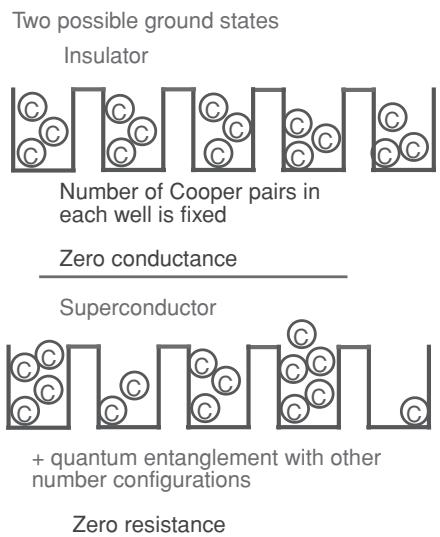
\includegraphics[width=0.5\textwidth]{figs/ch13/fig_13.11.jpg}
\caption*{图 13.11\quad 库珀对（C）的绝缘与超导基态，用以说明库珀对相位涨落与数量涨落之间的共轭性。在绝缘体中，库珀对数目的涨落停止，导致相位的无穷不确定。相反，在超导体中相位相干得以建立，从而使库珀对粒子数具有无穷的不确定性。}\label{fig:auto:13.11}
\end{figure}

在二维中把超导态转变为绝缘体的第二种手段，是从超导一侧施加垂直磁场（YK1995；MK1999；HP1990）。图 13.12 给出磁场调节的绝缘体--超导体转变中电阻率随温度的函数关系。磁场超过临界值后，库珀对被摧毁，绝缘行为通过单粒子局域化的方式出现。同样，在这两相的分界线（separatrix）上电阻率与温度无关。然而，这批数据令人惊讶之处在于：在“超导”一侧，低温下电阻率出现明显的变平（见图 13.12 插图）。也就是说，电阻率并未像超导体所预期的那样继续降到零，而是趋于饱和（YK1995；E1996）。在厚度调节的转变中也观察到了同样的行为。电阻率不消失表明相位相干的缺失。相位涨落在 $d=2$ 中特别强，众所周知它会拓宽电阻率赖以降到零的温度区间。此外，垂直磁场会产生称为涡旋（库珀对的对偶）的电阻性激发，它们阻挠全局相位相干的出现。尽管如此，尚无任何理论能够充分解释：当温度趋于零时，“超导”一侧的电阻率为何表观上并不消失。事实上，就在撰写本书之际，超导侧可能存在一个居间金属相（MK1999），仍是绝缘体--超导体领域悬而未决的核心问题。

\begin{figure}[H]\centering
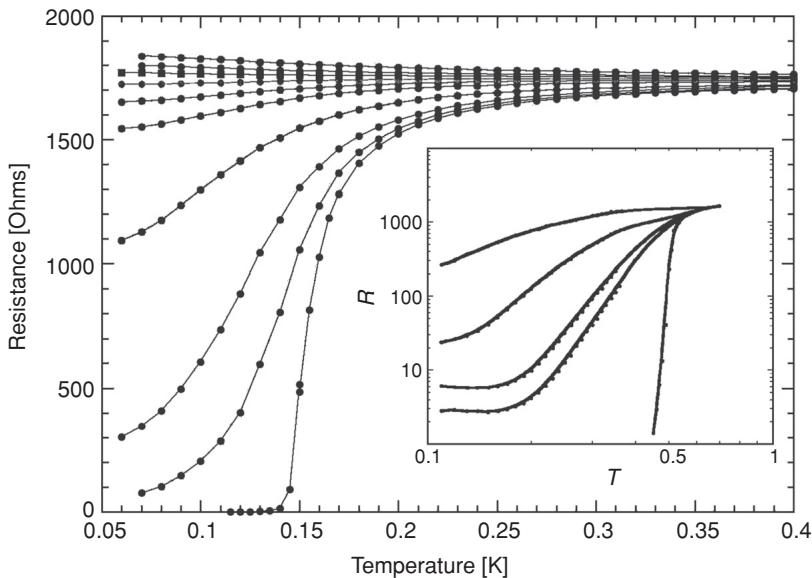
\includegraphics[width=0.65\textwidth]{figs/ch13/fig_13.12.jpg}
\caption*{图 13.12\quad MoGe 薄膜的电阻随温度的变化，磁场为 $B=0,0.5,1.0,2.0,3.0,4.0,4.4,4.5,5.5,6$ kG。零场下样品在 0.15 K 变为超导体；当磁场大于约 4.4 kG 时样品变为绝缘体。磁场低于该值但不为零时，电阻出现饱和。饱和行为在插图中另一个转变温度更高的样品上显示得更为清楚，插图给出 $B=0,1.5,2,4$ 和 7 kOe 的数据；更高磁场下该样品为绝缘体。数据取自 A. Yazdani 和 A. Kapitulnik, \emph{Phys. Rev. Lett.} \textbf{74}, 3037 (1995)。}\label{fig:auto:13.12}
\end{figure}

\subsection{稀薄电子气中的导电态}

局域化的最后一个例外，是平面内运动的电子带来的又一项惊讶。在揭示新导电相可能存在的实验中，调节参量是载流子的浓度（K1996；PFW1997；S1998；H1998）。电子（或空穴）被限制在两种半导体的界面上作横向运动，如硅金属--氧化物--半导体场效应晶体管（MOSFET）中的情形；或被限制在量子阱中，如 GaAs 的情形。在这两种体系中，电子密度都通过调节栅极上的偏压来控制。对电子（空穴）而言，偏压越正（负），电子密度越高。这类器件与研究量子霍尔效应所用的器件完全相同（见第 15 章）。如图 13.13 所示，当电子密度缓慢增加到约 $10^{11}/\mathrm{cm}^{2}$ 以上时，随着温度降低，电阻率从上升（绝缘行为）变为下降，这是导电行为的标志。在这两个极限之间的转变处，电阻率几乎与温度无关。尽管电阻率在零温下最终取什么值仍不清楚，但超过某一密度后电阻率的显著下降完全出乎意料，更重要的是，没有任何理论预言过它。然而，我们能否正确地断言零温下存在于两个不同物相之间的转变，仍未有定论。尽管如此，这些数据确实具有量子相变（如绝缘体--超导体转变）所共有的一个特征（S1999），即标度不变性。在这里，标度不变性只是意味着图 13.13 中平坦区以上的数据彼此相似；对平坦区以下的数据同样如此。于是，只要用同一个依赖于密度的标度因子去标度每条曲线，各种密度下的上、下两族电阻率曲线便都能坍缩到仅仅两条不同的曲线上。所得两条曲线的斜率符号相反，如图 13.13 的插图所示。此处出现的指数乘积，即关联长度（或局域化长度）指数与动力学指数 $z$ 的乘积。在量子相变中，能标在临界点上按 $\Omega\propto\xi^{-z}$ 消失。除非两相在零温下电学上截然不同，否则这种标度行为难以得到调和。

\begin{figure}[H]\centering
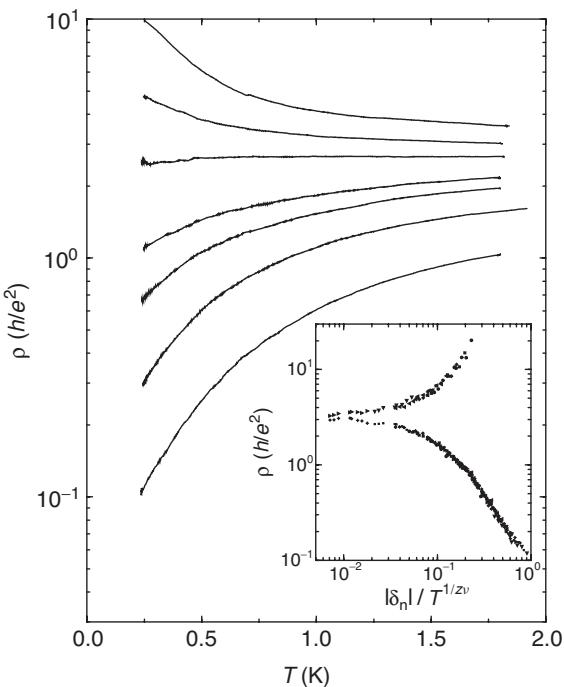
\includegraphics[width=0.55\textwidth]{figs/ch13/fig_13.13.jpg}
\caption*{图 13.13\quad 硅中二维电子气的电阻率（$\rho$）随温度的变化，磁场为零，电子密度 $n$ 各不相同（自上而下：0.86、0.88、0.90、0.93、0.95、0.99 和 $1.10\times 10^{11}/\mathrm{cm}^{2}$）。插图显示数据在临界转变密度（$n_{\mathrm{c}}$）上下坍缩为两条不同的标度曲线。此处 $\delta=(n-n_{\mathrm{c}})/n_{\mathrm{c}}$，$z=0.8$，$\nu=1.5$。}\label{fig:auto:13.13}
\end{figure}

刻画这一转变的关键实验特征（SK1999）如下：（1）存在临界电子或空穴密度 $n_{\mathrm{c}}$，导电相在其上出现；（2）存在一个特征温度，典型值为费米温度 $T_{\mathrm{F}}$ 的一半的量级，低于它时导电侧的电阻率大致按 $\rho_{1}+\rho_{0}(T)$ 下降，其中 $\rho_{0}(T)\approx\rho_{0}\exp(-T_{0}/T)$；（3）在绝缘相--导电相转变附近存在临界标度，预示着量子临界点；（4）非线性的电流--电压（I--V）曲线；（5）导电相被面内磁场与磁性杂质所压制；（6）一旦施加垂直磁场，新导电相便连续演化为某个量子霍尔态。

目前对这些现象尚无公认的解释。事实上，有人提出最终并不存在转变，电阻率的下降其实是一个制冷问题；也许起作用的是与硅的细节有关的物理（PF2005），而非源自电子相互作用的非微扰效应。无论这个问题的最终答案是什么，这些实验都有助于把注意力集中到稀薄电子气的基态上。我们确定地知道：在高密度与超低密度下，二维电子气都会被无序局域化。这两个区域由电子间库仑相互作用相对于其动能的大小来区分。如第 6 章所讨论，由于库仑相互作用按 $1/r$ 衰减（$r$ 为电子间距离），而动能按 $1/r^{2}$ 衰减，库仑相互作用在低密度下占主导。因此，在高密度区，电子本质上无相互作用，按安德森局域化原理的断言出现绝缘行为。在动能几乎为零的超低密度区，库仑相互作用主导物理。在这个极限下，电子彼此尽可能远离以使库仑相互作用最小，形成晶体排列，即维格纳晶体；它会被任意微量的无序钉扎，因而是绝缘体。新的导电相恰恰位于维格纳极限与非相互作用区之间。如图 13.14 所示，这一密度区是固体物理尚未攻克的疆域之一，因为当载流子浓度增大、维格纳型晶体被摧毁时所得到的基态究竟是什么，我们还没有任何确定的了解。我们把费米液体区的终点放在压缩率变号并变为负值的 $r_{\mathrm{s}}$ 处（见习题 9.6）。实验上，向导电态的转变伴随着压缩率的变号（DJ2000；I2000）。负压缩率是稀薄电子体系中常见的一种失稳，它标志着均匀密度态的不稳定性。然而，若补偿电荷背景是刚性的，离子便无法移动去促成非均匀的电子态，因此这一电荷失稳不会实现。在硅 MOSFET 与 GaAs 实验之前，曾有人预期如果二维中真能存在金属相，它应当出现在微扰区（$r_{\mathrm{s}}\ll 1$）（LR1985）。然而情形似乎并非如此：新的导电相恰恰出现在非微扰区，在那里无法先验地（\emph{a priori}）假定费米液体理论成立。

\begin{figure}[H]\centering
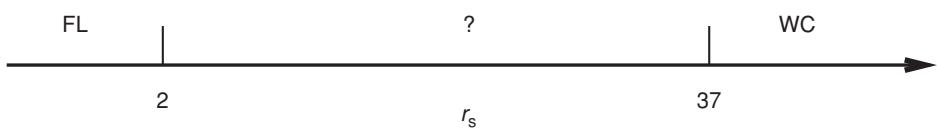
\includegraphics[width=0.7\textwidth]{figs/ch13/fig_13.14.jpg}
\caption*{图 13.14\quad 二维电子气的密度区间，以及对各区间确定知道的性质。低密度时形成维格纳晶体（WC），高密度时出现费米液体（FL）。这两个相都被无序局域化。维格纳晶体熔化边界已由 B. Tanatar 和 D. Ceperley 确定（\emph{Phys. Rev. B} \textbf{39}, 5005 (1989)）。新的导电相位于这两个区间之间。尚不清楚在这一区间内形成的是何种物态。}\label{fig:auto:13.14}
\end{figure}

维格纳晶体与其关联的近亲——莫特绝缘体——有一类相似之处。关于莫特绝缘态的原始论证（M1949）基于单电子原子构成的晶格。每个格点的单占据产生一个半满能带，后者通常允许电子自由导电。然而，莫特提出，随着晶格间距增大，交叠可以急剧减小，以致电子能带退化为局域的原子态。在这个极限下，每个原子都是中性的，因而不可能有电荷输运；尽管如此，能带仍是半满的。因此，与维格纳晶体一样，莫特绝缘态出现在库仑效应主导的稀薄区。

以莫特绝缘体为代表的稀薄电子体系容易发生诸多失稳，其中最著名的是超导电性。例如，整个有机导体家族（M1997）与铜氧化物高温超导体（A1992）在未掺杂时都是莫特绝缘体；掺杂后，两类材料都变为超导体。事实上，这看起来是一条实验事实：由层状材料构成的掺杂莫特绝缘体，在电荷有序态或自旋有序态附近表现出超导电性。为何出现这样的局面，至今仍是固体物理学中经久不消的难题之一。依此类比，有人提出（P1998；BK1998）处于维格纳晶体熔化边界附近的二维电子气应当毫无二致。但这一提议很可能与实验无关，因为在新的导电相中没有迹象表明电荷载体是 $2e$ 而非 $e$。显然，要查明稀薄二维电子气中金属态的最终成因，还需要进一步的实验。

\section*{小结}
\addcontentsline{toc}{section}{小结}

局域化源于相位相干的背散射。这类过程导致电子回归概率非零，从而在 $d\le 2$ 时不存在金属态。施加磁场或引入二聚体型的近邻关联，可以抵消无序使电子态局域化的自然倾向。然而，这些看似毫不相干的效应却有一个共同的起源。就磁场而言，时间反演这一分立对称性的破缺减小了电子背散射对电导率的贡献。在无规二聚体模型中，拥有对称面的缺陷所导致的透射共振使反射波即背散射波消失。正是背散射的完全缺失，在 RDM 类型的模型中给出了长程输运。局域化的其他例外出现在二维并涉及电子相互作用。这两个问题目前在实验上与理论上都尚未解决。

\section*{习题}
\addcontentsline{toc}{section}{习题}

\textbf{习题 13.1}\quad 考虑一线性链，在第 $m$ 个格点上放置一个缺陷。设格点幅为 $c_{n}$，$W$ 为缺陷的强度，线性链由如下演化方程描述：
\begin{equation*}
E c_{n}=\epsilon c_{n}+V(c_{n+1}+c_{n-1})+W\delta_{nm}c_{m}.\tag{13.45}
\end{equation*}
利用缺陷方法证明：当 $W\neq 0$ 时，单个束缚态在连续带之外形成。为实施该方法，采用如下步骤：（1）将本征值方程乘以 $\mathrm{e}^{\mathrm{i}kn}$ 并对 $n$ 求和；（2）再将所得方程乘以 $\mathrm{e}^{-\mathrm{i}km}$ 并积分，得到束缚态位置的判据
\begin{equation*}
1=W\langle G(E)\rangle,\tag{13.46}
\end{equation*}
其中
\begin{equation*}
\langle G(E)\rangle=\frac{1}{2\pi}\int_{-\pi}^{\pi}\frac{\mathrm{d}k}{E-\epsilon(k)}\tag{13.47}
\end{equation*}
且 $\epsilon(k)=\epsilon+2V\cos k$。证明：若 $W>0$，束缚态位于带之上，即能量 $E>\epsilon+2V$；而当 $W<0$ 时，束缚态位于带之下。对 $d=2$ 重复同样的计算。

\textbf{习题 13.2}\quad 在磁场存在时，电导率的总变化 $\delta(H)-\delta(H=0)$ 依赖于 $P_{H}$ 与 $P_{H=0}$ 之差。利用式 (13.20) 计算这一差值，并用式 (13.16) 对结果积分。定义 $x=2HD_{0}\tau_{\mathrm{in}}/c$ 作为磁场强度的量度。证明：当 $x\ll 1$ 时，$\Delta(H)\propto H^{2}\tau_{\mathrm{in}}^{2}$；在相反极限 $x\gg 1$ 下，证明 $\Delta(H)\propto\ln(H\tau_{\mathrm{in}})$。

\textbf{习题 13.3}\quad 证明 RDM 的非对角对偶（见图 13.9(c)）中的扩展态，与完美布洛赫态仅在每个缺陷格点处相差一个乘性因子 $V/\tilde{V}$。

\textbf{习题 13.4}\quad 把式 (13.34) 中的求和转换为积分，计算薄膜（$d=2$）与导线（$d=1$）的电导率。你应分别得到式 (13.35) 与式 (13.36)。

\textbf{习题 13.5}\quad 假定在欧姆区，$\beta$ 函数的一般形式为
\begin{equation*}
\beta=d-2-\frac{A_{d}}{g}.\tag{13.48}
\end{equation*}
在区间 $[L_{0},L]$ 上积分此量，分别得到 $d=1$ 与 $d=3$ 时电导对长度的显式依赖。证明：只要 $\epsilon=d-2\ll 1$，就有 $s=1$。

\section*{参考文献}
\addcontentsline{toc}{section}{参考文献}

\begin{itemize}[leftmargin=2em,itemsep=0pt,parsep=0pt,label={}]
\item [AAT1973] R. Abou-chacra, P. W. Anderson, and D. J. Thouless, \emph{J. Phys. C} \textbf{6}, 1734 (1973).
\item [A1979] E. Abrahams, P. W. Abrahams, D. C. Licciardello, and T. V. Ramakrishnan, \emph{Phys. Rev. Lett.} \textbf{42}, 673 (1979).（译注：第二作者原书印作 P. W. Abrahams，应为 P. W. Anderson。）
\item [A1981] S. Alexander, J. Bernasconi, W. R. Schneider, and R. Orbach, \emph{Rev. Mod. Phys.} \textbf{53}, 175 (1981).
\item [A1980] B. L. Altshuler, A. G. Aronov, D. E. Khmel'nitskii, and A. I. Larkin, in \emph{Quantum Theory of Solids}, ed. I. M. Lifshits (MIR Publishers, Moscow, 1980).
\item [A1958] P. W. Anderson, \emph{Phys. Rev.} \textbf{109}, 1492 (1958).
\item [A1992] P. W. Anderson, \emph{Science} \textbf{256}, 1526 (1992).
\item [BK1998] D. Belitz and T. R. Kirkpatrick, \emph{Phys. Rev. B} \textbf{58}, 8214 (1998).
\item [B1999] V. Bellani, E. Diez, R. Hey, \emph{et al.}, \emph{Phys. Rev. Lett.} \textbf{82}, 2159 (1999).
\item [B1982] G. Bergmann, \emph{Phys. Rev. B} \textbf{25}, 2937 (1982).
\item [BG1995] M. A. Blachly and N. Giordano, \emph{Phys. Rev. B} \textbf{51}, 12537 (1995).
\item [B1963] R. E. Borland, \emph{Proc. R. Soc. London Ser. A} \textbf{274}, 529 (1963).
\item [B1992] A. Bovier, \emph{J. Phys. A} \textbf{25}, 1021 (1992).
\item [DO1979] G. J. Dolan and D. D. Osheroff, \emph{Phys. Rev. Lett.} \textbf{43}, 721 (1979).
\item [DJ2000] S. C. Dultz and H. W. Jiang, \emph{Phys. Rev. Lett.} \textbf{84}, 4689 (2000).
\item [DWP1990] D. H. Dunlap, H.-L. Wu, and P. Phillips, \emph{Phys. Rev. Lett.} \textbf{65}, 88 (1990).
\item [EC1970] E. N. Economou and M. H. Cohen, \emph{Phys. Rev. Lett.} \textbf{24}, 1445 (1970).
\item [E1996] D. E. Ephron, A. Yazdani, A. Kapitulnik, and M. Beasley, \emph{Phys. Rev. Lett.} \textbf{76}, 529 (1996).
\item [FFG1955] G. Feher, R. C. Fletcher, and E. A. Gere, \emph{Phys. Rev.} \textbf{100}, 1784 (1955).
\item [F1990] M. P. A. Fisher, G. Grinstein, and S. Girvin, \emph{Phys. Rev. Lett.} \textbf{64}, 587 (1990).
\item [F1989] J. C. Flores, \emph{J. Phys. Condens. Matt.} \textbf{1}, 8471 (1989).
\item [GM1998] A. M. Goldman and N. Markovic, \emph{Physics Today} \textbf{51}, 39 (1998).
\item [H1998] Y. Hanien, U. Meirav, D. Shahar, \emph{et al.}, \emph{Phys. Rev. Lett.} \textbf{80}, 1288 (1998).
\item [HP1990] A. F. Hebard and M. A. Paalanen, \emph{Phys. Rev. Lett.} \textbf{65}, 927 (1990).
\item [I2000] S. Ilani, A. Yacoby, D. Mahalu, and H. Shtrikman, \emph{Phys. Rev. Lett.} \textbf{84}, 3133 (2000).
\item [I1986] Y. Imry, \emph{Europhys. Lett.} \textbf{1}, 249 (1986).
\item [J1989] H. M. Jaeger, D. B. Haviland, B. G. Orr, and A. M. Goldman, \emph{Phys. Rev. B} \textbf{40}, 182 (1989).
\item [JK1986] R. Johnston and B. Kramer, \emph{Z. Phys. B} \textbf{63}, 273 (1986).
\item [K1996] S. V. Kravchenko, D. Simonian, M. P. Sarachik, W. Mason, and J. E. Furneaux, \emph{Phys. Rev. Lett.} \textbf{77}, 4938 (1996).
\item [LN1966] J. S. Langer and T. Neal, \emph{Phys. Rev. Lett.} \textbf{16}, 984 (1966).
\item [LR1985] P. A. Lee and T. V. Ramakrishnan, \emph{Rev. Mod. Phys.} \textbf{57}, 287 (1985).
\item [LT1975] D. C. Licciardello and D. J. Thouless, \emph{J. Phys. C} \textbf{8}, 4157 (1975).
\item [LG1987] J. J. Lin and N. Giordano, \emph{Phys. Rev. B} \textbf{35}, 1071 (1987).
\item [MWP1997] I. Martin, Y. Wan, and P. Phillips, \emph{Phys. Rev. Lett.} \textbf{78}, 114 (1997).
\item [MK1999] N. Mason and A. Kapitulnik, \emph{Phys. Rev. Lett.} \textbf{82}, 5341 (1999).
\item [M1997] R. H. McKenzie, \emph{Science} \textbf{278}, 820 (1997).
\item [MJW1997] P. Mohanty, E. M. Q. Jariwala, and R. A. Webb, \emph{Phys. Rev. Lett.} \textbf{78}, 3366 (1997).
\item [M1949] N. F. Mott, \emph{Proc. Phys. Soc. London Sect. A} \textbf{62}, 416 (1949).
\item [M1972] N. F. Mott, \emph{Phil. Mag.} \textbf{26}, 1015 (1972).
\item [MT1961] N. F. Mott and W. D. Twose, \emph{Adv. Phys.} \textbf{10}, 107 (1961).
\item [M1990] K. A. Muttalib, \emph{Phys. Rev. Lett.} \textbf{65}, 745 (1990).
\item [P1987] J. B. Pendry, \emph{J. Phys. C} \textbf{20}, 733 (1987).
\item [P1993] P. Phillips, \emph{Ann. Rev. Phys. Chem.} \textbf{44}, 115 (1993).
\item [P1998] P. Phillips, Y. Wan, I. Martin, S. Knysh, and D. Dalidovich, \emph{Nature} \textbf{395}, 253 (1998).
\item [PF2005] A. Punnoose and A. M. Finkel'stein, \emph{Science} \textbf{310}, 289 (2005).
\item [PFW1997] D. Popovic, A. B. Fowler, and S. Washburn, \emph{Phys. Rev. Lett.} \textbf{79}, 1543 (1997).
\item [S1999] S. Sachdev, \emph{Quantum Phase Transitions} (Cambridge University Press, Cambridge, 1999).
\item [SK1999] M. P. Sarachik and S. V. Kravchenko, \emph{Proc. Natl. Acad. Sci.} \textbf{96}, 5900 (1999).
\item [S1998] M. Y. Simmons, A. R. Hamilton, M. Peppe, \emph{et al.}, \emph{Phys. Rev. Lett.} \textbf{80}, 1292 (1998).
\item [SE1984] C. M. Soukoulis and E. N. Economou, \emph{Phys. Rev. Lett.} \textbf{52}, 565 (1984).
\item [T1982] G. A. Thomas, Y. Ootuka, S. Katsumoto, S. Kobayashi, and W. Sasaki, \emph{Phys. Rev. B} \textbf{25}, 4288 (1982).
\item [T1977] D. J. Thouless, \emph{Phys. Rev. Lett.} \textbf{39}, 1167 (1977).
\item [VW1980] D. Vollhardt and P. W\"{o}lfle, \emph{Phys. Rev. Lett.} \textbf{45}, 482 (1980).
\item [W1976] F. Wegner, \emph{Z. Phys. B} \textbf{25}, 327 (1976).
\item [WGP1992] H.-L. Wu, W. E. Goff, and P. Phillips, \emph{Phys. Rev. B} \textbf{45}, 1623 (1992).
\item [YK1995] A. Yazdani and A. Kapitulnik, \emph{Phys. Rev. Lett.} \textbf{74}, 3037 (1995).
\end{itemize}
